%\documentclass[3p,times]{elsarticle}
%\usepackage{ecrc}
\documentclass[preprint,3p]{elsarticle}
\usepackage{graphicx}
% used for flow charts
\usepackage{listings}
\usepackage{pgf}
\usepackage{tikz}
\usepackage{reotex}
\usepackage{array}
\usepackage{algorithm}
\usepackage{algorithmic}
\usepackage{amssymb}
\usepackage{amsmath}
\usepackage{amsthm}

\usepackage[normalem]{ulem}
\usepackage{todonotes}
\usepackage{color}
\usepackage{verbatim}
\usepackage{listings}

%\usetikzlibrary{external}
%\tikzexternalize[prefix=figures/]
%\tikzset{external/force remake}

%\newcommand{\redt}[1]{\textcolor{red}{#1}}
\newcommand{\liyi}[1]{\textcolor{blue}{#1}}
\newcommand{\xy}[1]{{#1}}

\newtheorem{example}{Example}[section]
\newtheorem{theorem}{Theorem}[section]
\newtheorem{lemma}{Lemma}[section]

\lstset{
    basicstyle=\ttfamily\small,
    numbers=left,
    numberstyle=\small,
    columns=flexible,
    numbersep=10pt,
    tabsize=2,
    extendedchars=true,         %
    breaklines=true,
    keywordstyle=\bfseries,
    stringstyle=\color{white}\ttfamily, % Farbe der String
    xleftmargin=20pt,
    framexleftmargin=17pt,
    framexrightmargin=5pt,
    framexbottommargin=4pt,
    showstringspaces=false
    % frame=single
}

\lstdefinelanguage{coq}{
    keywords = {
        Parameter, Parameters, Variable, Variables,
        Fixpoint,
        Definition,
        Stream, Prop,
        forall, exists,
        Axiom, Lemma, Goal, Theorem,
        Proof, Qed,
        Hypothesis, Section,
    }
}

\renewcommand{\ttdefault}{pxtt}

\usepackage{url}


\journal{Science of Computer Programming}

%\pagestyle{plain}
\begin{document}
\begin{frontmatter}
%\pagestyle{plain}
%\mainmatter

\title{Reasoning about Connectors Using Coq and Z3}

%\titlerunning{Reasoning about Connectors in Coq}

\author{Xiyue Zhang}\ead{zhangxiyue@pku.edu.cn}
\author{Weijiang Hong}\ead{wj.hong@pku.edu.cn}
\author{Yi Li}\ead{liyi$\_$math@pku.edu.cn}
\author{Meng Sun}\ead{sunmeng@math.pku.edu.cn}
\address{LMAM \& DI, School of Mathematical Science, Peking University, Beijing, China}
%\email{\{zhangxiyue,wj.hong,liyi\_math,sunm\}@pku.edu.cn}}

%\maketitle
\begin{abstract}
Reo is a channel-based exogenous coordination language in which complex coordinators, called connectors, are compositionally built out of simpler ones. In this paper, we present an approach to model and reason about connectors using Coq and Z3.
Both models reflect the original structure of connectors \liyi{as closely as possible}. In our framework, both basic connectors (channels) and composition operations are \xy{modeled as axioms.} Furthermore, complex connectors are modeled as the combination of logical predicates which correspond to simpler connectors. With such definitions provided, connector properties, as well as equivalence and refinement relations between different connectors, can be formalized as \emph{goals} in Coq and proved using pre-defined \emph{tactics}, if satisfied by connectors. \xy{When failing to prove whether a property is satisfiable or not with Coq, we use Z3, an SMT solver, to search for possible bounded counter examples automatically.}
% Particularly, to fulfill the proof of refinement relation, Z3 is used as an assistant tool for solving logical formulas.
%\paragraph*{Keywords:}

\end{abstract}
\begin{keyword}
Coordination language, Reo, Coq, Z3, Reasoning
\end{keyword}
\end{frontmatter}
\section{Introduction}\label{sec:introduction}

Modern software systems are typically distributed over large networks of \xy{computing devices.} \xy{Usually the components}
that comprise a system do not exactly fit together as pieces of a jigsaw puzzle, but leave significant interfacing gaps
that must somehow be filled with additional code. Compositional coordination models and languages provide a formalization
of the ``glue code" that interconnects the constituent \liyi{components, organizes} the mutual interactions \xy{between them} in a
distributed processing environment, and \xy{plays} a crucial role for the success of component-based systems in the past decades.

As an example,  \xy{Reo \cite{Arb04} is a channel-based exogenous coordination language, that offers
a powerful framework for implementation of coordinating component connectors.} Connectors provide the protocols that control and organize
the communication, synchronization and cooperation among the components that they interconnect. Primitive connectors, called {\em channels}
in Reo, can be composed to build complex connectors. Reo has been successfully applied in different application domains, such as
service-oriented computing and bioinformatics \cite{CCA04, SA07}. \xy{In recent years,
verifying the correctness of connectors is becoming a critical challenge, especially due to the advent of Cloud computing
technologies. The rapid \liyi{growth in size} and complexity of the computing infrastructures leads to more complex structure of connectors, makes it more difficult to model
and verify connector properties, and thus decreases the confidence on the correctness of connectors.}


Several works have been done for formal modeling and \xy{verification of connectors.} An operational semantics for Reo using Constraint Automata
(CA) was provided by Baier et al. \cite{BSAR06}, and later the symbolic model checker Vereofy \cite{BBK+10} was developed,
which can be used to check CTL-like properties.
% However, modeling unbounded primitives or even bounded primitives with unbounded
% data domains is impossible with finite constraint automata. Bounded large data domains cause an
% explosion in the constraint automata model which becomes problematic.
% A model for Reo connectors based on the idea of coloring a connector with possible data flows to
% resolve synchronization and exclusion constraints was presented by Clarke et al. \cite{CCA07}. Unlike the operational semantics,
% data sensitive behavior, which is supported by Reo, are not captured by the coloring approach.
Besides, one attractive approach is \xy{to translate Reo} to other formal models such as Alloy
\cite{KSA+08}, mCRL2 \cite{KKV12}, UTP \cite{AAA+09,SAA+12}, etc.,
which makes it possible to take advantage of existing verification
tools. A comparison of existing semantic models for Reo can be found
in \cite{JA12}.

In a previous paper \cite{ZHL+17} we showed how to formally model and reason about connectors' properties in Coq. The basic idea of our approach is to model the behavior of \xy{a connector as a logical predicate} which describes the relation among the timed data streams on the input and output nodes, and to reason about connectors' properties, as well as the equivalence and refinement relations between connectors, by using proof principles and tactics in Coq. \xy{Almost all existing approaches for modeling and verification of Reo connectors are state-based or automata-based, in which the automata for complex connectors are constructed through product operation on simpler ones. As a result, the number of states of connectors  may grow exponentially, which makes it inefficient and even impossible to verify connector properties in model checkers. Compared with existing approaches for verifying connectors' properties \cite{BBK+10,KB09,KKV12}, reasoning about connectors using theorem provers like Coq is especially helpful when we take infinite behavior into consideration. The coinductive proof principle makes it possible to prove connectors' properties easily while it is difficult (sometimes impossible) for other approaches (like model checking) because of the huge (or maybe infinite) number of states.}

The approach in this paper is not a brand new idea, as we have already provided a solution for modeling Reo in Coq in \cite{LS15}, where connectors are represented in a constructive way, and verification is essentially based on simulations. We do believe that the approach in this paper is reasonably different from its predecessor \cite{LS15} where Coq seldom shows its real power. To be more specific, this work has its certain
advantages comparing with \cite{LS15} in the following aspects:
\begin{itemize}
\item {\bf Modeling Method:} We use axioms to describe basic channels and their composition operations, which is more natural on a proof-assistant platform than the simulation-based approach in \cite{LS15}.
\item {\bf Expressive power:} Any valid Coq expression can be used to depict properties, which is obviously more powerful than just using LTL formulas in \cite{LS15}. \liyi{Then}, \xy{support for continuous time behavior is also possible in our approach in this paper as we make use of real numbers to represent time values.}
\end{itemize}

\xy{
  This paper is an extension of out earlier work \cite{ZHL+17} where equivalence and refinement relations can be proved among different connectors, while the approach in \cite{LS15} is not capable of either equivalence or refinement checking.
  In the current paper, we aim to provide a more complete approach to formally model and reason about Reo connectors compared with the approach in \cite{ZHL+17}. The main drawback in \cite{ZHL+17} is that \liyi{sometimes the user fails} to prove that the complementary refinement relation holds or not using Coq. This problem is partially made up by using Z3 \cite{MouraB08} in this paper. While Coq provides a platform to prove properties with a series of tactics and strategies to be considered, Z3 can be used as a component that \liyi{can build automatically counter-examples when the properties do not hold}. The logical formulas involved in the \liyi{Reo models} should \liyi{reflect, in the same way as the Coq model, the} constraints of connectors and be consistent with their behavior.
  % Adopting the Z3 SMT solver in this work makes it possible to automatically find bounded counter examples when the refinement relations do not hold.
}

The paper is organized as follows. After this general introduction, we briefly summarize Reo, Coq and Z3
in Section \ref{sec:pre}. Section \ref{sec:channelandoperator} introduces the
formal model of basic channels, operators and complex connectors in Coq. Section
\ref{sec:verification} shows how to reason about connector properties and equivalence (or
refinement) relations under our Coq formalization. Section \ref{sec:refinement} provides a Reo model in Z3 and shows the usage of Z3 in refinement checking.
In Section \ref{sec:conclusion}, we conclude with some further research directions. Full source codes \xy{are provided} at \cite{reo2coq2Z3} for further reference.

\section{Preliminaries}\label{sec:pre}

In this section, we provide a brief introduction to the coordination language Reo, \liyi{the Coq proof assistant} and the Z3 SMT solver.

\subsection{The Coordination Language Reo}
Reo is a channel-based exogenous coordination language \xy{where complex coordinators, called connectors,}
are compositionally built out of simpler ones \cite{Arb04}.
The simplest connectors are channels with well-defined behavior such as synchronous channels, FIFO channels, etc.
% Each channel in Reo has exactly two directed ends, with their own identities.
There are two types of channel ends: \emph{source} ends and \emph{sink} ends. A source channel end accepts
data into the channel, and a sink channel end dispenses data out of the channel.
\begin{figure}
  \centering
  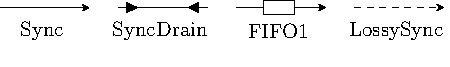
\includegraphics[width=.5\textwidth]{basics.pdf}
  \caption{Four types of basic channels.}\label{fig:basicchannel}
\end{figure}

The graphical notations of some basic channels are presented in Figure~\ref{fig:basicchannel}, and their behavior can be interpreted as follows:
\begin{itemize}
\item{\textbf{Sync:} a synchronous channel with one source end and one sink end. The pair of I/O operations on its two ends \xy{can only succeed simultaneously.}}
\item{\textbf{SyncDrain:} a synchronous channel which has two source ends.
 The pair of input operations on its two ends \xy{can only succeed} simultaneously.
 All data items written to this channel are lost.}
\item{\textbf{FIFO$n$:} an asynchronous channel with one source end and one sink end, and a bounded buffer with capacity $n$.
It can \xy{accept $n$ data items from its source end before emitting data on its sink end.} The accepted data items are kept in the internal buffer, and dispensed to
the sink end in FIFO order.
Especially, the FIFO$1$ channel is an instace of FIFO$n$ where the buffer capacity is 1.}
%\item{\textbf{AsyncDrain:}  an asynchronous channel} which has two source ends. The channel guarantees that the operations on its two ends never succeed simultaneously. All data items written to this channel are lost.
\item{\textbf{LossySync:} a synchronous channel with one source end
    and one sink end. The source end always accepts all data items. If
    there is no matching output operation on the sink end of the
    channel at the time that a data item is accepted, then the data
    item is lost; otherwise, the channel transfers the data item
    as a Sync channel, and the output operation at the sink end succeeds.}
\end{itemize}

\begin{figure}[ht]
\centering
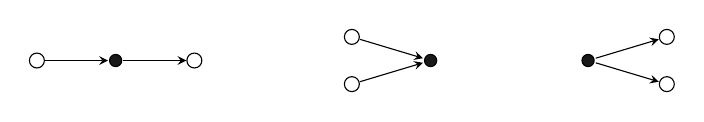
\begin{tikzpicture}
  \ionode{(io1)}{(0,5)}{}
  \ionode{(io2)}{(2,5)}{}
  \ionode{(io3)}{(4,4.7)}{}
  \ionode{(io4)}{(4,5.3)}{}
  \ionode{(io5)}{(8,4.7)}{}
  \ionode{(io6)}{(8,5.3)}{}
  \mixednode{(m1)}{(1,5)}{}
  \mixednode{(m2)}{(5,5)}{}
  \mixednode{(m3)}{(7,5)}{}
  \sync{(io1)}{(m1)}{}
  \sync{(m1)}{(io2)}{}
  \sync{(io3)}{(m2)}{}
  \sync{(io4)}{(m2)}{}
  \sync{(m3)}{(io5)}{}
  \sync{(m3)}{(io6)}{}
\end{tikzpicture}
\caption{Operations of channel composition.}\label{fig:channelcomposition}
\end{figure}

Complex connectors are constructed by composing simpler ones \xy{via the \emph{join} and \emph{hiding} operations.} Channels are joined together in nodes. The set of channel ends coincident on a node is disjointly partitioned into the sets of source and sink channel ends that coincide on the node, respectively. Nodes are categorized into source, sink and mixed nodes, depending on whether all channel ends that coincide on a node are source ends, sink ends or a combination of the two. The hiding operation is used to hide the internal topology of a connector. The hidden nodes can no longer be accessed or observed from outside. There are three types of operations for channel composition: \emph{flow-through}, \emph{merge} and \emph{replicate}. Figure~\ref{fig:channelcomposition} provides the graphical representation of these operations. \xy{Further details about Reo and its semantics can be found in \cite{Arb04, AR03, BSAR06}.}

\subsection{Coq and Z3}

Coq \cite{huet1997coq} is a widely-used \xy{proof assistant, where denotational formalizations (e.g.
theorem and hypothesis) and operational ones} (e.g. functions and algorithms) are naturally
integrated. Moreover, it allows the interactive construction of formal proofs.
The formal language used in Coq, \emph{Gallina}, provides a convenient way to define
both programming statements and mathematical propositions, for example:
\begin{lstlisting}[language=coq]
(* a variable definition *)
Variables a b: nat.
(* a simple non-recursive function *)
Definition inc(a:nat) := a + 1.
(* axioms don't have to be proved *)
Axiom inc_ax: forall c:nat, inc(c) > c.
(* theorems rely on proving *)
Theorem inc_eq: forall c:nat, inc(c) = c + 1.
Proof.
(* interactive proving based on tactics *)
auto.
Qed.
\end{lstlisting}
As shown in this example, \xy{there are two different modes} in Coq's interactive shell. When
we start Coq, we can write declarations and definitions in a functional-programming mode. Then, when
we start a \emph{Theorem}, or \emph{Lemma}, Coq jumps into the proving mode. We need to \xy{write
\emph{tactics} }to reduce the proving goal and finally finish the formal proof.

\xy{Coq is equipped with a set of well-written standard libraries. }For example, as used in
this paper, \emph{Stream} provides a co-inductive
definition of infinite lists, and \emph{Reals} defines various operations and theorems on real
numbers. Usually, quite a few lemmas and theorems are pre-defined in such libraries, making it
substantially easier to prove our goals.

%An abstract term has a type descriptor but no implementation, which is denoted as \emph{variables}
%or \emph{parameters}. Usually such terms are used to define theorems, e.g.
%\begin{verbatim}
  %Variables A B: Prop.
  %Theorem the: A -> B.
  %Proof.
    %...
  %Qed.
%\end{verbatim}
%In Contrast, an concrete term is more like a traditional function, e.g.
%\begin{verbatim}
  %Definition func(a:nat):nat := a + 1.
%\end{verbatim}
%An interesting feature of Coq is that both abstract and concrete terms can be unified in the same
%framework. For example, we can use \emph{Variable} to declare a function with no implementations.
%And such definitions are exactly equivalent with a proposition when both the arguments and the
%results are propositions. Similarly, a proof term, of a theorem of lemma, is a concrete term whose
%type is equal to the theorem.

%Besides, Coq provides a series of impressive libraries. For example, both \emph{Streams} and
%\emph{Reals} are already well-defined in Coq's standard library. Based on their work, we can prove
%many propositions more easily.


Z3 \cite{MouraB08} is an efficient SMT (Satisfiability Modulo Theories) solver freely available from Microsoft. It \liyi{has been} used in various software verification and analysis applications. \xy{Z3 expands to deciding the satisfiability }(or dually the validity) of first order formulas with respect to combinations of theories such as: arithmetic, bit-vectors, arrays, and uninterpreted functions. Given the data and time constraints of connectors, \xy{it allows us to verify the satisfiability \liyi{of} properties or refinement relations.} Z3 provides bindings for several programming languages. In this paper, we use \emph{Z3 python-bindings} to construct the models and carry out experiments. The following example provides an intuitive understanding of the Z3 solver.
\begin{lstlisting}
x, y = Int('x'), Int('y')

s = Solver()
s.add(x > 10, Or(x + y > 3, x - y < 2))
# Checking satisfiability of constraints in the solver s
print s.check()

# Create a new scope
s.push()
s.add(y < 11)
# Checking satisfiability of updated set of constraints
print s.check()

# Restoring state
s.pop()
# Checking satisfiability of restored set of constraints
print s.check()
\end{lstlisting}

This example contains two constraints at first. From these two constraints, \xy{we can see that Z3 supports operators like $<$, $>$ for comparison, apart from boolean operators, such as \emph{And}, \emph{Or}, \emph{Not} and \emph{Implies}.}
The function \emph{Solver} creates a general purpose solver instance where constraints can be asserted through its \emph{add} method. The method \emph{check} \liyi{assesses the satisfiability of the} asserted constraints. \xy{Finally, the result is satisfiable (unsatisfiable) if the solver returns \emph{sat} (\emph{unsat}) respectively.} A solver may fail to \liyi{check the satisfiability of} a system of constraints and \emph{unknown} is returned. Each solver maintains a stack of assertions. The command \emph{push} creates a new scope by saving the current stack size. The command \emph{pop} removes all constraints that have been asserted after the last \emph{push} command.


\section{Formal Modeling in Coq}\label{sec:channelandoperator}
In this section, we show how primitive connectors, i.e., channels, and operators for connector composition are specified in Coq and used for \xy{modeling complex connectors. }Basic channels, which can be regarded as axioms of the whole framework, are specified as logical predicates illustrating the relation between the timed data streams of input and output. When we need to construct a more complex connector, appropriate composition operators are applied depending on the topological structure of the connector.

\subsection{Basic Definitions}\label{sec:basicdef}

% In this section, we briefly introduce the notion of timed data streams and some pre-defined auxiliary functions and predicates in Coq, which are used in the following sections for modeling connectors.

%\subsection{Timed data streams}
The behavior of a connector can be formalized by means of data-flows at its sink and source nodes which are essentially infinite sequences. With the help of the stream library in Coq, such infinite data-flows can be defined as \emph{timed data streams}:
\begin{lstlisting}[language=coq]
Definition Time := R.
Definition Data := nat.
Definition TD := Time * Data.
Variable Input : Stream TD.
Variable Output : Stream TD.
\end{lstlisting}
%
In our framework, time is represented by real numbers. %Benefit from the completeness of real number system, we can express and carry out the effective operation of a quantity at any precision request.
The continuity of the set of real numbers is sufficiently enough for our modeling approach. Also the
continuous time model is more appropriate than the discrete model since it is very expressive and closer to the nature of time in the real world. \xy{Thus, the time sequence consists of increasing and diverging time moments.} For simplicity, here we take the natural numbers as the definition of data, which can be easily expanded according to different application domains. The Cartesian product of time and data defines a TD object.
We use the stream module in Coq to produce streams of TD objects.

%\subsection{Auxiliary functions and predicates}
Some auxiliary functions and predicates are defined to \liyi{ease} the representation of axioms for basic channels in Reo. This part can be extended for further use in different problems.
The terms \emph{PrL} and \emph{PrR} take a pair of values (a, b) that has Cartesian product type A $\times$ B as the argument and return the first or second value of the pair, respectively.
%\begin{verbatim}
%    Definition PrL {A B: Type}(pair: A * B) := (...).
%    Definition PrR {A B: Type}(pair: A * B) := (...).
%\end{verbatim}
The following functions provide some judgment of time, which can make
the description of axioms and theorems for connectors more concise and
clear: \emph{Teq} \xy{means that values of time in \liyi{the two streams taken as parameters} are equal} and \emph{Tneq} has the
opposite meaning. \emph{Tle}  (\liyi{resp.} \emph{Tgt}) represents that time of the first stream is
strictly \liyi{lesser} (greater) than the second stream. The judgement about
equality of data is analogous to the judgement of time. \xy{\emph{Deq} represents that the data of two streams are equal.}The complete
definition of these functions can be found at \cite{reo2coq2Z3}.

\subsection{Formal Modeling of Basic Channels}

\xy{We use the previous predicates} to describe the constraints on time and data, respectively, \xy{and their conjunction} to provide the complete specification of basic channels. \xy{This approach provides a relational semantics for Reo using predicates that relates the inputs and outputs of connectors.} This model offers convenience for the analysis and proof of connector properties. In the following, we present a few examples of the formal model of basic channels.

The simplest form of a synchronous channel is denoted by the Sync channel type. For a channel of the Sync type, a read operation on
its sink end succeeds only if there is a write operation pending on its source end. Thus, the time and data of a stream flowing
into the channel are exactly the same as the stream that flows out of the channel
\footnote{If we use $\alpha,\beta$ to denote the data streams that flow through the channel ends of a channel and $a,b$ to denote the time stream corresponding to the data streams, i.e., the $i$-th element $a(i)$ in $a$ denotes exactly the time moment of the occurrence of $\alpha(i)$, then we can easily obtain the specifications for different channels, as discussed in \cite{Sun12,SAA+12}. For example, a synchronous channel can be expressed as $\alpha=\beta \wedge \emph{a}=\emph{b}$.}.
The Sync channel can be defined as follows in the Coq system:
\begin{lstlisting}[language=coq]
Definition Sync (Input Output:Stream TD) : Prop :=
    Teq Input Output /\ Deq Input Output.
\end{lstlisting}


The channel of type SyncDrain is a synchronous channel that allows pairs of write operations pending on its two ends to succeed simultaneously. All written data items are lost. Thus, the SyncDrain channel is used for synchronising two timed data streams on its two source ends. This channel type is an important basic synchronization building block for the construction of more complex connectors. The SyncDrain channel can be defined as follows:
\begin{lstlisting}[language=coq]
Definition SyncDrain (Input Output:Stream TD) : Prop :=
    Teq Input Output.
\end{lstlisting}


The channel types FIFO and FIFO$n$ where $n$ is an integer \liyi{strictly greater} than $0$ represent the
typical unbounded and bounded asynchronous FIFO channels. A write to a FIFO channel always succeeds, and a write to a FIFO$n$ channel succeeds only if the
number of data items in its buffer is less than its bounded capacity $n$. A read or take operation on a FIFO or FIFO$n$ channel suspends until the first data item
in the channel buffer can be obtained and then the operation succeeds.
%We use the $\overrightarrow{\emph{a}}$ to denote the tail of  a sequence \emph{a}.
For simplicity, we take the FIFO1 channel as an example. This channel type requires that the time when it consumes a data item through its source end is \liyi{strictly earlier} than the time when the data item is delivered through its sink end. Besides, as the buffer has the capacity 1, time of the next data item that flows in should be \liyi{strictly later} than the time when the data in the buffer is delivered. We use \xy{the conjunction of predicates} in its definition as follows:
\begin{lstlisting}[language=coq]
Definition FIFO1(Input Output:Stream TD) : Prop :=
    Tle Input Output /\ Tle Output (tl Input) /\ Deq Input Output.
\end{lstlisting}

For a FIFO1 channel whose buffer already contains a data element \emph{e}, the communication can be initiated only if the data element \emph{e} can be taken via the sink end. In this case, the data stream that flows out of the channel should get an extra element \emph{e} settled at the beginning of the stream. And time of the stream that flows into the channel should be \liyi{strictly earlier} than time of the tail of the stream that flows out. But as the buffer contains the data element \emph{e}, new data can be written into the channel only after the element \emph{e} has been taken. Therefore, time of the stream that flows out is \liyi{strictly earlier} than time of the stream that flows in. The channel can be represented as:
\begin{lstlisting}[language=coq]
Definition FIFO1e(Input Output:Stream TD)(e:Data) : Prop :=
    Tgt Input Output /\ Tle Input (tl Output)
    /\ PrR (hd Output) = e  /\ Deq Input (tl Output).
\end{lstlisting}

In the following we \liyi{define LossySync as an Axiom}
because it is easier to use than the coinductive \liyi{expression that specifies its behavior}.

A LossySync channel behaves the same as a Sync channel, except that a write operation on its source end always succeeds immediately. If a compatible read or take operation is already pending on its sink end, the written data item is transferred to the pending operation and both succeed. Otherwise, the write operation succeeds and the data item is lost. The LossySync channel can be defined as follows:
\begin{lstlisting}[language=coq]
Parameter LossySync: Stream TD -> Stream TD -> Prop.
Axiom LossySync_coind:
    forall Input Output: Stream TD,
    LossySync Input Output ->
    (( hd Output = hd Input  /\ LossySync (tl Input)(tl Output)) \/
       LossySync(tl Input) Output).
\end{lstlisting}

% AsyncDrain is analogous to SyncDrain except that it guarantees that the pairs of write operations on the two channel ends never succeed simultaneously. Similarly it only has requirements on the time of the two streams on its opposite ends, but it requires that the times of the two streams are always different. The AsyncDrain channel can be defined as follows:
% \begin{lstlisting}[language=coq]
% Parameter AsyncDrain: Stream TD -> Stream TD -> Prop.
% Axiom AsyncDrain_coind:
%     forall Input1 Input2: Stream TD,
%     AsyncDrain Input1 Input2 ->
%     (~ PrL(hd Input1)  =  PrL (hd Input2) ) /\
%     (
%         ( (PrL(hd Input1) < PrL (hd Input2)) /\ AsyncDrain (tl Input1) Input2) /\
%         ( (PrL(hd Input1) > PrL (hd Input2))  /\ AsyncDrain Input1 (tl Input2) )
%     ).
% \end{lstlisting}

%Note that in the above definitions we choose Axiom to define LossySync and AsyncDrain
%because it is easier to use the coinductive expression to specify their behavior.

\xy{Defining basic channels by conjunction and disjunction of predicates provides the following benefits:}
\begin{itemize}
\item Firstly, \liyi{this makes the structure of the definition in Coq identical to the usual implementation}.
\item Secondly, we can easily split predicates for proofs of different properties which can make the proving process simpler.
\end{itemize}
%Each predicate can be viewed as an atom. The theorems and propositions which will be described later are also illustrated by atomic expressions.

\subsection{Formal modeling of Operators}
\xy{We have shown the formalization of channel types in Coq}. Now we start defining the composition operators for connector construction. \xy{There are three types of composition operators}, which are \emph{flow-through}, \emph{replicate} and \emph{merge}, respectively.

The flow-through operator simply allows data items to flow through the junction node, from one channel to the other. \xy{We do not need to give the flow-through operator a specific definition in Coq as this operator can be achieved directly through renaming of nodes.} For example, \xy{while we specify} two channels \emph{Sync(A,B)} and \emph{FIFO1(B,C)}, a flow-through operator that acts on node \emph{B} for these two channels has been \xy{achieved implicitly by using the same identifier.}

%The property of replicate operator in Reo can be seen in the composition of two channels \emph{ab},\emph{cd}.
The replicate operator puts the source ends of different channels together into one common node, and a write operation on this node succeeds only if all the channels are \liyi{able to consume} a copy of the written data. %And the two channel ends are interchangeable.
\xy{Similar to the flow-through operator, the replicate operator can be directly achieved through renaming of nodes according to the structure of connectors, i.e. \liyi{making all the nodes connected by the replicate operator having the same name}.} For example, for two channels \emph{Sync(A,B)} and \emph{FIFO1(C,D)}, we can illustrate \emph{Sync(A,B)} and \emph{FIFO1(A,D)} in Coq instead of defining a function like \emph{rep(Sync(A,B),FIFO1(C,D))} and the replicate operator is achieved directly by renaming \emph{C} with \emph{A} for the FIFO1 channel.

The merge operator is more complicated. We consider merging two
channels \emph{AB} and \emph{CD}. When the merge operator acts on
these two channels, it leads to a choice of taking from the common
node that delivers a data item out of \emph{AB} or \emph{CD}.
\xy{The first predicate is related to the time constraint. We require that data items \liyi{from the two source ends} cannot come at the same time.
Similar to the definition of basic channels, we define merge as the conjunction of predicates and use recursive definition here:}
%    Definition xor(a b: Prop) :=  (a \/ b) /\ ~(a /\ b).
\begin{lstlisting}[language=coq]
Parameter merge: Stream TD -> Stream TD ->Stream TD -> Prop.
Axiom merge_coind:
    forall s1 s2 s3:Stream TD,
    merge s1 s2 s3-> (
    ~ (PrL(hd s1) = PrL(hd s2)) /\
    ( (PrL(hd s1) < PrL(hd s2)) -> ((hd s3 = hd s1)  /\ merge (tl s1) s2 (tl s3)) ) /\
    ( (PrL(hd s1) > PrL(hd s2)) -> ((hd s3 = hd s2)  /\ merge s1 (tl s2) (tl s3)) )
    ).
\end{lstlisting}

\begin{figure}
\vspace{0cm}
\centering
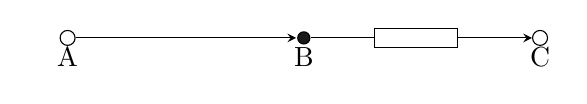
\begin{tikzpicture}
\ionode{(io1)}{(0.5,0)}{node[below]{A}}
\ionode{(io2)}{(6.5,0)}{node[below]{C}}
\mixednode{(m1)}{(3.5,0)}{node[below]{B}}
\sync{(io1)}{(m1)}{}
\fifoe{(m1)}{(io2)}{}
\end{tikzpicture}
\caption{A connector consisting of a Sync channel and a FIFO1 channel.}\label{fig:compsyncfifo}
\end{figure}

Based on the definition of basic channels and operators, more complex connectors can be constructed structurally.
%As the whole structure of each connector has been determined, the rest work is to use the operators to connect appropriate  channels according to the structure of each connector.
To show how a composite connector is constructed, we consider a simple example as shown in Figure \ref{fig:compsyncfifo}, where a FIFO1 channel is attached
to the sink end of a Sync channel. Assume \emph{AB} is of type Sync and \emph{BC} is of type FIFO1, then we can construct the required connector by
illustrating \emph{Sync(A,B)} and \emph{FIFO1(B,C)}. The configuration and the functionality of the required connector can be specified using this concise method. Note that the composition operations can be easily generalized to the case of multiple nodes, where the modeling of connectors is similar. More
examples can be found in Section \ref{sec:verification}.






\section{Reasoning about Connectors in Coq}\label{sec:verification}
After modeling a connector in Coq, we can analyse and prove important properties of the connector. In this section, we give some examples to elucidate how to
reason about connector properties and prove refinement/equivalence \xy{relations between different connectors }with the help of Coq.


\subsection{Derivation of Connector Properties}
The proof process of a property is as follows: the user states the proposition that needs to be proved, called a \emph{goal},
\xy{and then he/she} applies commands called \emph{tactics} to decompose this goal into simpler subgoals or \liyi{prove} it directly. This decomposition
process ends when all subgoals are completely \liyi{proved}. In the following, \xy{we use four examples} to illustrate our approach instead of
giving all the complex technical details.
\begin{example}
We first consider the connector given in Figure \ref{fig:compsyncfifo}, which consists of two channels \emph{AB} and \emph{BC} with types Sync and FIFO1, respectively.
We use $a$ and $b$ to denote the time streams when the corresponding data streams \liyi{flow in and out of} the Sync channel \emph{AB}, and
$c$ to denote the time stream for the data stream that flows out of the FIFO1 channel \emph{BC}. Here we can see that \liyi{flow-through
behavior is performed} by the mixed node \emph{B}. The time when the stream flows into the FIFO1 channel \emph{BC} is equal to the time when the
stream flows out of the Sync channel \emph{AB}. The following theorem states the property $a < c$ for this connector. The connector is based on the
axioms Sync and FIFO1, which can be used as hypotheses for the proof of the following theorem.
\end{example}

\begin{theorem}[Transfer\_le]\label{the:tleac}
$\forall A,B,C.\:Sync(A,B)\land FIFO1(B,C) \rightarrow Tle(A,C)$.
\end{theorem}

In Coq, the theorem can be proved as follows:
\begin{lstlisting}[language=coq]
Theorem thm_4_1: forall A B C,
  Sync A B /\ FIFO1 B C -> Tle A C.
Proof.
    intros. destruct H. destruct H0.
    intro n. rewrite H. apply H0.
Qed.
\end{lstlisting}

First we give the Coq system a proposition
\texttt{thm\_4\_1} which needs to be proved. The proposition is represented by a logical expression.
Table \ref{test1} shows the detailed \liyi{proof steps} and the feedback that the Coq system provides during the proof.
\begin{table}
\small
\renewcommand{\arraystretch}{1.2}
\newcommand{\tabincell}[2]{\begin{tabular}{@{}#1@{}}#2\end{tabular}}
  \centering
  \begin{tabular}{|>{\tt}c|c|c|}\hline
\tabincell{c}{Step} & \tabincell{c}{Feedback}
\\\hline
\tabincell{c}{Theorem thm\_4\_1:\\\emph{forall A B C,} \\ \emph{Sync A B $\rightarrow$ FIFO1 B C}
   \emph{$\rightarrow$  Tle A C.}} & \tabincell{c}{ 1 subgoal:\\ \emph{forall A B C,} \\ \emph{Sync A B $\rightarrow$ FIFO1 B C  $\rightarrow$ Tle A C} } \\\hline
\tabincell{c}{intros } & \tabincell{c}{ 1 subgoal: \emph{Tle A C} \\ \emph{H : Sync A B;
H0 : FIFO1 B C}} \\\hline
\tabincell{c}{destruct \emph{H} } & \tabincell{c}{ 1 subgoal:  \emph{Tle A C} \\ \emph{H : Teq A B;
H1 : Deq A B;}  \\ \emph{H0 : FIFO1 B C}} \\\hline
\tabincell{c}{destruct \emph{H0} } & \tabincell{c}{ 1 subgoal: \emph{Tle A C} \\ \emph{H : Teq A B;
H1 : Deq A B;}\\ \emph{
H0 : Tle B C; H2 : Tle C (tl B$)\wedge D$eq B C }}\\ \hline
\tabincell{c}{intro \emph{n} } & \tabincell{c}{ 1 subgoal: \emph{PrL (Str\_nth n A) $<$ PrL (Str\_nth n C)} \\ \emph{H : Teq A B;
H1 : Deq A B;
H0 : Tle B C; }\\
\emph{H2 : Tle C (tl B$)\wedge D$eq B C}} \\\hline
\tabincell{c}{rewrite \emph{H}} & \tabincell{c}{ 1 subgoal: \emph{PrL (Str\_nth n B) $<$ PrL (Str\_nth n C) }\\ \emph{H : Teq A B;
H1 : Deq A B;
H0 : Tle B C;}\\
\emph{H2 : Tle C (tl B)$\:\wedge\:$Deq B C;
n : nat}} \\\hline
\tabincell{c}{apply \emph{H0} } & \tabincell{c}{ No more subgoals} \\\hline
\end{tabular}

\caption{Steps and feedbacks for proving Theorem \ref{the:tleac}}\label{test1}
\end{table}

\xy{The aforementioned benefits of using conjunction and disjunction of logical predicates to describe basic channels instead of formalizing them based on automata or states have emerged while proving this example.}
After constructing the new connector, we use \texttt{intros} to split conditions and conclusions. Then we can use \texttt{destruct} to obtain the conditions for time and data separately,
and make the proving procedure much more convenient. \xy{Once we obtain the concrete conditions, we can use \texttt{intro} to reduce the subgoal to the comparison between each time point in these two sequences.} Then by using \texttt{rewrite H}, we can make
the proof a step forward with known conditions of the comparison of time \emph{a} and \emph{b}, and finally by
\texttt{apply H0} we can prove the goal. This is the implementation for reasoning about the constructed connector.
Note that proper selection of strategies and tactics is essential for the proof of connector properties.


\begin{example}\label{ex:alternator}
In this example, we show a more interesting connector named \emph{alternator} which consists of three channels \emph{AB}, \emph{AC} and \emph{BC} of type SyncDrain, FIFO1 and Sync, respectively. With the help of this connector, we can get data from node \emph{B} and \emph{A} alternatively at node \emph{C}.
By using the axioms for the basic channels and operators of composition, we can get the connector as shown in Figure \ref{fig:alternator}(b). The two
channels \emph{AC} and \emph{BC} are merged together at node \emph{C}. Before the merge operation, the connector's structure is as shown in
Figure \ref{fig:alternator}(a), which is useful in the reasoning about the alternator.

Here the replicate operation has been applied twice for the alternator: node \emph{A} becomes the common source node of \emph{SyncDrain (A,B)} and \emph{FIFO1(A,C1)}, and node \emph{B} becomes the common source node of \emph{SyncDrain(A,B)} and \emph{Sync(B,C2)}. Let the time streams when the
data streams flow \liyi{in the} two source nodes \emph{A} and \emph{B} be denoted by $a$ and $b$, and the time streams when the data streams
flow out of the channels \emph{FIFO1(A,C1)} and \emph{Sync(B,C2)} be denoted by $c1$ and $c2$, respectively. Theorem \ref{the:alternator}
specifies the property $c2<c1 \wedge c1<tl (c2)$ of the connector in Figure \ref{fig:alternator}(a). The connector is based on the axioms
Sync, SyncDrain and FIFO1. These three corresponding axioms are used as hypotheses for the proof of this theorem.
\end{example}

\begin{figure}
\vspace{0.5cm}
\centering
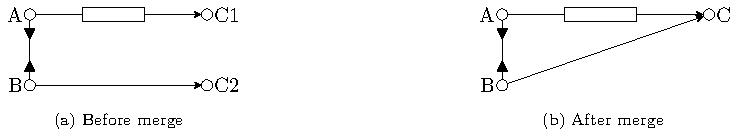
\includegraphics[width=.8\textwidth]{alternator.pdf}
\caption{Alternator}
\label{fig:alternator}
\end{figure}

\begin{theorem}[Unmerge]\label{the:alternator}

$\forall A,B,C1,C2\,.\,
SyncDrain(A,B)\land FIFO1(A,C1)\land Sync(B,C2)  \rightarrow Tle(C2,C1) \wedge Tle(C1, tl(C2))
$
\end{theorem}

We first introduce some lemmas to \liyi{ease} the proof.
\begin{lstlisting}[language=coq]
Lemma transfer_eq : forall s1 s2 s3 : Stream TD
  ((Teq s1 s2) /\ (Teq s2 s3)) -> (Teq s1 s3).
Lemma transfer_eqtl : forall s1 s2 : Stream TD,
  (Teq s1 s2) -> (Teq tl s1)) (tl s2)).
Lemma transfer_leeq : forall s1 s2 s3 : Stream TD,
  ((Tle s1 s2) /\ (Teq s2 s3)) -> (Tle s1 s3).
Lemma transfer_hdle : forall s1 s2 : Stream TD,
  (Tle s2 s1) -> (PrL (hd s1) > PrL (hd s2)).
\end{lstlisting}

In Coq, the theorem can be proved as follows. Note that the formalism is slightly different from the previous one. \liyi{The \emph{section} environment encapsulate} hypotheses as assumptions of the theorem. So the two definitions are exactly equivalent.

\begin{lstlisting}[language=coq]
Section Alt.
Hypothesis D1: SyncDrain A B.
Hypothesis D2: FIFO1 A C1.
Hypothesis D3: Sync B C2.
Theorem unmerge:
   (Tle C2 C1)  /\  (Tle C1 (tl C2)).
\end{lstlisting}

After constructing the connector in Figure \ref{fig:alternator}(a), we use \texttt{destruct} to obtain the conditions for time and data, respectively.
\xy{Because the goal we are going to prove} is \liyi{the} conjunction of logical predicates, we use \texttt{split} to obtain the single subgoals represented by logical predicates. \xy{Further, \texttt{intros} is used to reduce the goal into the \liyi{element-wise} comparison between each data in these two sequences.} Then \texttt{rewrite} and \texttt{apply} are
used similarly multiple times until the goal is proved finally. %We can see that a new tactic named \emph{split} is used in the proof of
%this property.
Concrete proof steps and feedbacks are specified in Table \ref{tb:proof}.

\begin{table}[H]
\newcommand{\tabincell}[2]{\begin{tabular}{@{}#1@{}}#2\end{tabular}}
  \centering
  \small
  \renewcommand{\arraystretch}{1.2}
  \begin{tabular}{|>{\tt}c|c|c|}\hline
\tabincell{c}{Step} & \tabincell{c}{Feedback}\\\hline
\tabincell{c}{Theorem unmerge%:\\((Tle C2) C1) $\wedge$ ((Tle C1) (tl C2))
}
   & \tabincell{c}{ 1 subgoal: \emph{Tle C2 C1 $\wedge$ Tle C1 (tl C2)}} \\\hline
\tabincell{c}{destruct \emph{D2} } & \tabincell{c}{ 1 subgoal: \emph{Tle C2 C1 $\wedge$ Tle C1 (tl C2)}
 \\ \emph{H : Tle A C1;
H0 : Tle C1 (tl A) $\wedge$ Deq A C1}} \\\hline
\tabincell{c}{destruct \emph{D3} } & \tabincell{c}{ 1 subgoal: \emph{Tle C2 C1 $\wedge$ Tle C1 (tl C2)}
 \\\emph{H : Tle A C1;
H0 : Tle C1 (tl A) $\wedge$ Deq A C1;}\\
\emph{H1 : Teq B C2;
H2 : Deq B C2}} \\\hline
\tabincell{c}{
destruct \emph{H0}} & \tabincell{c}{ 1 subgoal: \emph{Tle C2 C1 $\wedge$ Tle C1 (tl C2)}
\\\emph{H : Tle A C1;
H0 : Tle C1 (tl A);}\\
\emph{H3 : Deq A C1;
H1 : Teq B C2;
H2 : Deq B C2}} \\\hline
\tabincell{c}{split } & \tabincell{c}{2 subgoals: \emph{Tle C2 C1; Tle C1 (tl C2)}\\ \emph{H : Tle A C1;
H0 : Tle C1 (tl A);}\\
\emph{H3 : Deq A C1;
H1 : Teq B C2;
H2 : Deq B C2}} \\\hline
\tabincell{c}{intros $n$ } & \tabincell{c}{ 2 subgoals: \emph{PrL (Str\_nth n C2) $<$ PrL (Str\_nth n C1); Tle C1 (tl C2)} \\
\emph{H : Tle A C1;
H0 : Tle C1 (tl A);
H3 : Deq A C1;}\\
\emph{H1 : Teq B C2;
H2 : Deq B C2;
n : nat}
} \\\hline
\tabincell{c}{rewrite  $\leftarrow$ \emph{H1} } & \tabincell{c}{ 2 subgoals: \emph{PrL (Str\_nth n B) $<$ PrL (Str\_nth n C1); Tle C1 (tl C2)}\\
\emph{H : Tle A C1;
H0 : Tle C1 (tl A);
H3 : Deq A C1;}\\
\emph{H1 : Teq B C2;
H2 : Deq B C2;
n : nat}} \\\hline
\tabincell{c}{rewrite  $\leftarrow$ \emph{D1} } & \tabincell{c}{ 2 subgoals: \emph{PrL (Str\_nth n A) $<$ PrL (Str\_nth n C1); Tle C1 (tl C2)}\\
\emph{H : Tle A C1;
H0 : Tle C1 (tl A);
H3 : Deq A C1;}\\
\emph{H1 : Teq B C2;
H2 : Deq B C2;
n : nat}} \\\hline
\tabincell{c}{apply \emph{H} } & \tabincell{c}{ 1 subgoal: \emph{Tle C1 (tl C2)} \\ \emph{H : Tle A C1;
H0 : Tle C1 (tl A);
H3 : Deq A C1;}\\
\emph{H1 : Teq B C2;
H2 : Deq B C2}} \\\hline
\tabincell{c}{intros $n$ } & \tabincell{c}{ 1 subgoal: \emph{Tle C1 (tl C2)} \\ \emph{H : Tle A C1;
H0 : Tle C1 (tl A);
H3 : Deq A C1;}\\
\emph{H1 : Teq B C2;
H2 : Deq B C2}} \\\hline
\tabincell{c}{rewrite  $\leftarrow$ \emph{D4} } & \tabincell{c}{ 2 subgoals: \emph{PrL (Str\_nth n C1) $<$ PrL (Str\_nth n (tl B)); Teq B C2}\\
\emph{H : Tle A C1;
H0 : Tle C1 (tl A);
H3 : Deq A C1;}\\
\emph{H1 : Teq B C2;
H2 : Deq B C2;
n : nat}} \\\hline
\tabincell{c}{rewrite  $\leftarrow$ \emph{D5} } & \tabincell{c}{ 3 subgoals: \emph{PrL (Str\_nth n C1) $<$ PrL (Str\_nth n (tl A)); Teq A B; Teq B C2}\\
\emph{H : Tle A C1;
H0 : Tle C1 (tl A);
H3 : Deq A C1;}\\
\emph{H1 : Teq B C2;
H2 : Deq B C2;
n : nat}} \\\hline
\tabincell{c}{apply \emph{H0} } & \tabincell{c}{ 2 subgoals: \emph{Teq A B; Teq B C2} \\ \emph{H : Tle A C1;
H0 : Tle C1 (tl A);
H3 : Deq A C1;}\\
\emph{H1 : Teq B C2;
H2 : Deq B C2;
n : nat}} \\\hline
\tabincell{c}{apply \emph{D1} } & \tabincell{c}{ 1 subgoal: \emph{Teq B C2} \\ \emph{H : Tle A C1;
H0 : Tle C1 (tl A);
H3 : Deq A C1;}\\
\emph{H1 : Teq B C2;
H2 : Deq B C2;
n : nat}} \\\hline
\tabincell{c}{apply \emph{D3}} & \tabincell{c}{ No more subgoals.} \\\hline
\end{tabular}
\caption{Steps and feedback}\label{tb:proof}
\end{table}

%The proof of Theorem \ref{the:alternator} for the connector in Figure \ref{fig:alternator}(a) can be used to simplify the proof for the following property of alternator.

An additional hypothesis is needed for the proof of alternator which merges \emph{C1} and \emph{C2} into a common node \emph{C}. Based on the three
hypotheses for channels and \xy{the additional one}. \liyi{The alternation theorem} is presented as the following proposition which needs to be proved:
\begin{lstlisting}[language=coq]
Hypothesis D4: merge C1 C2 C.
Theorem alternator:
  hd C = hd C2 /\ merge C1 (tl C2) (tl C).
Proof.
  destruct unmerge.  (* ... *)
\end{lstlisting}
\xy{Here we only present the first step which shows how a proven theorem can be applied in another proof and omit the full details.
Note that the property of the unmerged alternator (i.e. Theorem \ref{the:alternator}) mentioned at the beginning of the example turns out to be very useful in the proof of the property of alternator. The unmerged alternator consists of three channels. \emph{AB}, \emph{AC1} and \emph{BC2} are of type SyncDrain, FIFO1 and Sync shown on the left side of Figure \ref{fig:alternator}. We construct the connector \emph{Alternator} through the unmerged one instead of building it from basic channels. As for verification, it also simplifies the process of proving the property of alternator as we can take advantage of the property of the unmerged one directly.}


\subsection{Refinement and Equivalence}

A refinement relation between connectors which \liyi{allows developing connectors systematically} in a step-wise fashion, may help to bridge
the gap between requirements and the final implementations. The notion of refinement has been widely used in different system descriptions.
For example, in data refinement \cite{RE98}, the `concrete' model is required to have \emph{enough redundancy} to represent all the elements
of the `abstract' one. This is captured by the definition of a surjection from the former into the latter (the \emph{retrieve map}). If
models are specified in terms of pre and post-conditions, the former are weakened and the latter strengthened under refinement \cite{Jon90}.
In process algebra, refinement is usually discussed in terms of several `observation' preorders, and most of them justify
transformations entailing \emph{reduction of nondeterminism} (see, for
example, \cite{Ros98}). For, the refinement relation can be
defined as in \cite{SAA+12}, where a proper refinement order over
connectors has been established based on the implication relation on
predicates.

%Based on our connector models in Coq, the implication relation on predicates establishes a proper refinement order over connectors.
%Generally speaking, a formal model \emph{A} refines another model \emph{B} means that \emph{B} contains more behavior than \emph{A}.
%Here we adopt the definition of refinement in \cite{SAA+12}.
\xy{Connector $Q$ is a refinement of another connector $P$ if the behavior property of $P$ can
be derived from \emph{hypothesis Q}, i.e., the \liyi{behavior property} of connector $Q$ (denoted by $P \sqsubseteq Q$). Two connectors are equivalent if each one of them is a refinement of the other.}
In the following, we show two examples of such refinement and equivalence relations for connectors.

\begin{example}[Refinement]
\label{ex:refine}
Taking the two connectors in Figure \ref{refine} into consideration, connector $Q$ is a refinement of connector $P$.
\begin{figure}
\vspace{0cm}
\centering
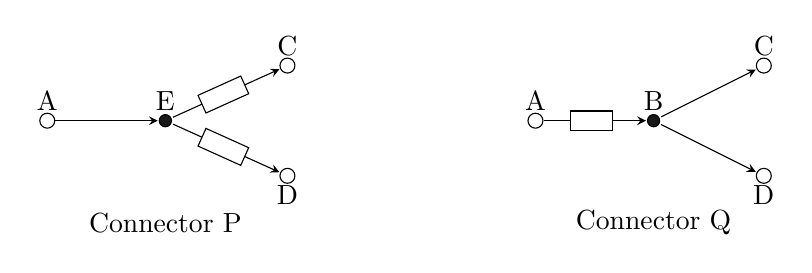
\begin{tikzpicture}
\ionode{(io4)}{(5,1.0)}{node[above]{A}}
\ionode{(io5)}{(7.9,1.7)}{node[above]{C}}
\ionode{(io6)}{(7.9,0.3)}{node[below]{D}}
\mixednode{(m2)}{(6.5,1.0)}{node[above]{B}}
\draw (6.5, -0.3) node[draw=none] {Connector Q};

\ionode{(io1)}{(-1.2,1.0)}{node[above]{A}}
\ionode{(io2)}{(1.85,1.7)}{node[above]{C}}
\ionode{(io3)}{(1.85,0.3)}{node[below]{D}}
\mixednode{(m1)}{(0.3,1.0)}{node[above]{E}}
\draw (0.3, -0.3) node[draw=none] {Connector P};


\sync{(io1)}{(m1)}{}
\fifoe{(m1)}{(io2)}{}
\fifoe{(m1)}{(io3)}{}

\sync{(m2)}{(io5)}{}
\sync{(m2)}{(io6)}{}
\fifoe{(io4)}{(m2)}{}
\end{tikzpicture}
\caption{Example of connector refinement}
\label{refine}
\end{figure}

We have mentioned that newly constructed connectors can be specified as theorems. Given arbitrary input timed
data stream at node \emph{A} and output timed data streams at nodes \emph{C}, \emph{D},
%essentially connector
%$Q$ is a refinement of another connector $P$ only if the behavior property of $P$ can
%be derived from \emph{theorem Q}, i.e., the property of connector $Q$.
connector $P$ enables the
data written to the source node \emph{A} to be asynchronously taken out via the two sink nodes \emph{C} and \emph{D}, but
it has no constraints on the relationship between the time of the two output events. On the other hand,
connector $Q$ refines this behavior by synchronizing the two sink nodes, which means that the two output
events must happen simultaneously. To be more precise, we use $c,d$ to denote the time streams of the two outputs
and $a$ to denote the time stream of the input. Connector $P$ satisfies condition $a<c\wedge a<d$ and
connector $Q$ satisfies $a<c\wedge a<d \wedge c=d$.
\end{example}

The refinement relation can be formally defined in Coq as:

%\begin{theorem}[refinement]
%$\forall A,C,D$:
%\begin{eqnarray*}
%\exists B. FIFO1(A,B)\wedge Sync(B,C)\wedge Sync(B,D) & \rightarrow & \\
%\exists E. Sync (A,E) \wedge FIFO1 (E,C) \wedge FIFO1 (E,D)
%\end{eqnarray*}
%\end{theorem}


\begin{lstlisting}[language=coq]
Theorem refinement : forall A C D,
    (exists B, (FIFO1 A B) /\ (Sync B C) /\ (Sync B D)) ->
    (exists E, (Sync A E) /\ (FIFO1 E C) /\ (FIFO1 E D)).
\end{lstlisting}


% Specifically, the refinement relation in this example can be formally represented as the following implication relation:
%  \begin{eqnarray*}
%    \forall B_{0}.FIFO1(A,B_{0})\wedge Sync(B_{0},C)\wedge Sync(B_{0},D) & \rightarrow &  \\
%    \exists B.Sync(A,B)\wedge FIFO1(B,C) \wedge FIFO1(B,D)
%  \end{eqnarray*}

To prove this refinement relation, we first introduce a lemma which is frequently used in the proof.
\begin{lemma}[Eq]\label{lemma:eq}
$\forall A,B: Stream~TD.\:Sync (A,B) \Leftrightarrow A = B$.
\end{lemma}
The lemma means that $Sync(A, B)$ and $A=B$ can be derived
from each other. Although this lemma seems to make the presence of
Sync channels in connectors redundant, it is not the case for most
connectors. For example, if we consider
the alternator in Example 2, it cannot accept any input data if we
remove the synchronous channel \emph{BC} and use one node for it.

By using the axioms for the basic channels and the operators of composition, we can obtain the two connectors easily.
In the process of constructing the connectors, the flow-through and replicate operations act once for each connector, respectively.


\begin{figure}[htbp]
\centering
\includegraphics[width=11.5cm]{Refinement.pdf}
\caption{Proof Steps Flow Chart}
\label{fig:equivalence}
\end{figure}

Figure \ref{fig:equivalence} shows the flow chart for the proof steps of
connector refinement in this example.


We now show the specific tactics used in the proof of refinement
$P \sqsubseteq Q$ for connectors $P$ and $Q$
in this example.
We need to find a timed data stream which specifies the data-flow through node \emph{E} of connector $P$, i.e., an appropriate \emph{$E$} that satisfies $Sync(A,E)\wedge FIFO1(E,C) \wedge FIFO1(E,D)$.

\liyi{First, we} employ \texttt{intros} to acquire a simpler subgoal $\exists E_{0}. Sync(A,E_{0})
\wedge FIFO1(E_{0},C) \wedge FIFO1(E_{0},D)$. Then we assert that $E=A$.
\liyi{After, using} \texttt{split}, we split the goal into two subgoals $Sync (A, E)$ and $FIFO1 (E, C) \wedge FIFO1 (E, D)$. \liyi{And, by \texttt{rewrite $H_{0}$} ($H_{0}: E = A)$} we replace the two subgoals with $Sync (A, A)$ and $FIFO1 (E, C) \wedge FIFO1 (E, D)$, respectively.

Through \texttt{apply} Lemma \ref{lemma:eq} (\emph{Eq}), we have $A = A$ in place of $Sync (A, A)$. Next the tactic \texttt{reflexivity} makes the subgoal $A = A$ proved directly. Up to now, the initial subgoal $Sync (A, E)$ has been achieved.

Using \texttt{split} again, the remaining unproven subgoal is split into two subgoals \emph{FIFO1 (E, C)} and \emph {FIFO1 (E, D)}.
After destructing the precondition three times, we succeed in obtaining three hypotheses: \emph{ H: FIFO1 (A, x); H1: Sync (x, C); H2: Sync (x, D)}. \liyi{Assuming} $x = C$ and then using tactics \texttt{apply Eq} and \texttt{assumption}, assertion $x = C$ is proved easily. Meanwhile, we get hypothesis \emph{H3: x $=$ C}. Via \emph{Rewrite $\leftarrow$H3}, we bring left in place of the right side of the equation \emph{H3: x = C} into \emph{FIFO1 (E, C)} and have \emph{FIFO1 (E, x)}. Similarly, \texttt{rewrite H0} and further we get the result \emph{FIFO1 (A, x)} which is exactly hypothesis \emph{H}. By using \texttt{assumption}, the second subgoal is proved already.
Using substantially the same tactic steps, \emph{FIFO1 (E, D)} can be proved. Finally, we have no more subgoals. %Note that there is a new tactic \texttt{reflexivity} used in the proof, which is actually synonymous with \texttt{apply refl equal}. We can use it to prove that two statements are equal.



\begin{example}[Equivalence]
%When connector $P$ is a refinement of  connector $Q$ and $Q$ is a refinement of $P$, we say that connector $P$ and $Q$ is equivalent.
For the connector $P$ in Example \ref{ex:refine}, we can add three more basic channels to build a new connector \emph{R} which is equivalent to $Q$. \emph{R} can be interpreted similarly based on basic channels and operators. We will omit the details for its construction here and prove the equivalence between the two connectors \emph{R} and $Q$ directly.
%The specific channels and operators used to construct the new connector will not be repeated here. Next we will prove the equivalence of the two connectors.
\end{example}

\begin{figure}[htb]
\vspace{0cm}
\centering
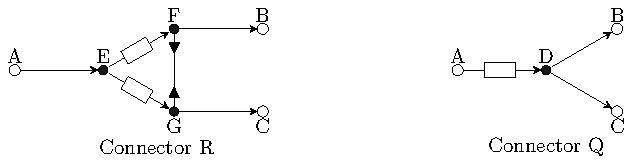
\includegraphics[width=.7\textwidth]{equivalence.pdf}
\caption{Example of connector equivalence}
\label{refine1}

\end{figure}

Equivalence relationship between the two connectors can be formalized as:
\begin{lstlisting}[language=coq]
Theorem equivalence: forall A B C,
  (exists E F G,
    (Sync A E) /\ (FIFO1 E F) /\ (Sync F B) /\
    (FIFO1 E G) /\ (Sync G C) /\ (SyncDrain F G)
  ) <->
  (exists D,
    (FIFO1 A D) /\ (Sync D B) /\ (Sync D C)
  ).
\end{lstlisting}
The proof of this theorem has two steps. Firstly, we prove that the new connector \emph{R} is a refinement of connector $Q$.
\liyi{We aim at finding} an appropriate \emph{$D$} that satisfies
\[
FIFO1(A,D)\wedge Sync(D,B) \wedge Sync(D,C)
\]
Similar to Example \ref{ex:refine}, we first assert $D=F$, which leads to
\[
FIFO1(A,F) \land Sync(F,B) \wedge Sync(F,C)
\]
From Lemma \ref{lemma:eq}, we have $Sync(A,E)$, or $A=E$. Therefore, \emph{FIFO1(E,F)} can be replaced by \emph{FIFO1(A,F)}. By adopting \emph{FIFO1(E,F)} and \emph{FIFO1(E,G)}, we can prove that the data sequences at \emph{F} and \emph{G} are equal. Similarly, data sequences at $C$, $G$ and $F$ are also equal, wrt. $Sync(G,C)$.

Further according to \emph{Sync(G,C)} and \emph{SyncDrain(F,G)}, the time sequences at \emph{F} and \emph{C} are proved equal. With the combination of relations on time and data between \emph{F} and \emph{C}, we can draw the conclusion \emph{Sync(F,C)}.


Up to now, we present a proof for \emph{Sync(F,C)} and \emph{FIFO1(A,F)} by the derivation. Besides, \emph{Sync(F,B)} is already declared in the assumptions. Consequently, the refinement relation has been proved.

Secondly, we prove that connector $Q$ is a refinement of connector \emph{R}.
We hope to find appropriate timed data streams at \emph{E,F,G}  which satisfy
\begin{eqnarray*}
\emph{Sync(A,E)}&\wedge& \emph{Sync(G,C)} \wedge \emph{FIFO1(E,G)}\wedge \emph{Sync(F,B)}\\
 &\wedge& \emph{FIFO1(E,F)}\wedge \emph{SyncDrain(F,G)}.
\end{eqnarray*}
We can directly assume $E=A$, $F=D$ and $G=D$. Now we only need to prove
$Sync(A,A) \wedge  Sync(D,C)  \wedge  FIFO1(A,D) \wedge  Sync(D,B) \wedge FIFO1(A,D) \wedge SyncDrain(D,D)$, which can be easily derived from the assumptions.


\section{Refinement Checking in Z3} \label{sec:refinement}
As shown previously, modeling and reasoning of Reo connectors in Coq allows us to reason about a relatively wide range of properties. \xy{However, when dealing with verification of refinement/equivalence relations between connectors, it is only capable of proving that one connector is indeed a refinement of the other one but cannot automatically provide a counter example when one connector is not a refinement of the other connector.} Moreover, the refinement relation is a fairly important part of properties, which has been investigated in many applications. \xy{When we fail to find a proof of the existence of refinement relations between connectors using Coq, we \liyi{propose to use} Z3, an SMT solver,}  to search for bounded counter examples. If a counter example is successfully located, it means that there is no refinement relation between the connectors.

\subsection{Formalization of Basic Channels in Z3}
\label{subsec:basicchannelsinZ3}

We first need to implement the construction of connectors and also define the refinement checking function in a way \xy{that fits Z3.} Typically, connector construction starts with the formal definition of basic channels and composition operators, \liyi{which will be used hereafter to build and assess more complex models. Such a framework must be carefully developed so that the further modeling can be simplified as much as possible}.

Coinciding with the definition of channels in Coq, we dealt with both time and data relation constraints in the basic definition. An auxiliary function \texttt{Conjunction} is used to take the conjunction of every constraint in the constraint lists parameterized by \emph{constraints}.
%By means of \texttt{Conjunction}, \xy{the definitions of basic channels are succinct.}
For example, the specific behavior constraints for \emph{Sync} channel are classified into two types: data constraints and time constraints. \liyi{The definition of \emph{Sync} in Coq provides} the behavior pattern it needs to follow: each item in timed data streams of output specified as ``node[1]'' is equivalent to the timed data items of input specified as ``node[0]'', which are exactly data and time constraints. As they are both requirements that we need to satisfy no matter data or time is related, each constraint in the list will all be combined finally.
%\lstset{language=Python}
\begin{lstlisting}
def Sync(nodes, bound):
   assert len(nodes) == 2
   constraints = []
   for i in range(bound):
     constraints += [ nodes[0]['data'][i] == nodes[1]['data'][i] ]
     constraints += [ nodes[0]['time'][i] == nodes[1]['time'][i] ]
   return Conjunction(constraints)
\end{lstlisting}

\emph{SyncDrain} channel is defined in a similar way. On the basis of the behavior of \emph{SyncDrain} channel, only time related constraints are needed, i.e., equivalence of corresponding items in two time streams of the two inputs.
\begin{lstlisting}
def SyncDrain(nodes, bound):
   assert len(nodes) == 2
   constraints = []
   for i in range(bound):
       constraints += [nodes[0]['time'][i] == nodes[1]['time'][i]]
   return Conjunction(constraints)
\end{lstlisting}

Regarding \emph{FIFO1} channel, data related constraints are the same as the \emph{Sync} channel. But there are different time related constraints for the \emph{FIFO1} channel. As the buffer capacity is one, the relations of each item in the input time stream and output time stream need to be carefully dealt with, \liyi{especially as} the next input should be \liyi{strictly later} than the present output. If the buffer contains a data item at the beginning, i.e. the variant version \emph{FIFO1e} channel, then the constraints related to data and time are just a little different. Note that the data item ``\emph{e}'' in the buffer should be the first one \liyi{to transit} and all the differences made to the constraints result from it. At last, their corresponding constraint lists consist of constraint statements similar to the statements above.
\begin{lstlisting}
def Fifo1(nodes, bound):
   assert len(nodes) == 2
   constraints = []
   for i in range(bound):
      constraints += [ nodes[0]['data'][i] == nodes[1]['data'][i] ]
      constraints += [ nodes[0]['time'][i] <  nodes[1]['time'][i] ]
      if i != 0:
          constraints += [ nodes[0]['time'][i] > nodes[1]['time'][i-1] ]
   return Conjunction(constraints)
\end{lstlisting}
\begin{lstlisting}
def Fifo1e(e):

  def Fifo1eInstance(nodes, bound):
    assert len(nodes) == 2
    constraints = []
    constraints += [nodes[1]['data'][0] == e]
    for i in range(bound-1):
        constraints += [nodes[0]['data'][i] == nodes[1]['data'][i + 1]]
        constraints += [nodes[0]['time'][i] < nodes[1]['time'][i + 1]]
    for i in range(bound):
        constraints += [nodes[0]['time'][i] > nodes[1]['time'][i]]
    return Conjunction(constraints)

  return Fifo1eInstance
\end{lstlisting}

In accordance with the behavior of \emph{LossySync} channel, each item of the input stream may or may not be lost. If a timed data item is lost, then the corresponding output gets nothing. If not, it behaves exactly like a successful transit of \emph{Sync} channel, so in this case the data and time related constraints are identical with those in the definition of \emph{Sync} channel. The biggest difference is that \emph{LossySync} channel should be defined in a recursive way according to its own distinctive behavior. Note that the constraints are added recursively which \liyi{coincides with} the original definition.
\begin{lstlisting}
def LossySync(nodes, bound, idx = 0, num = 0):
   assert len(nodes) == 2
   if bound == num:
     return True
   if bound == idx:
     return True
   constraints_0 , constraints_1 = [], []
   constraints_0 += [ nodes[0]['time'][idx] != nodes[1]['time'][num]]
   constraints_1 += [ nodes[0]['data'][idx] == nodes[1]['data'][num]]
   constraints_1 += [ nodes[0]['time'][idx] == nodes[1]['time'][num]]
   return Or(
     And(Conjunction(constraints_0), Channel.LossySync(nodes, bound, idx + 1, num)),
     And(Conjunction(constraints_1),  Channel.LossySync(nodes, bound, idx + 1, num + 1))
   )
\end{lstlisting}
\subsection{Composition Operators}\label{sec:compoperatorZ3}
While the basic channels are already well defined as the basis of the whole construction framework, the composition operators also need to be specified for large-scale connectors' construction just like cement for bricks. There are three kinds of composition operators: \emph{replicate}, \emph{flow-through} and \emph{merge}.

Both \emph{replicate} and \emph{flow-through} operators can be implicitly achieved when we compose channels to construct connectors using same node names. A simple example for the implementation of \emph{replicate} is \texttt{c1.connect('Sync', 'A', 'E'), c1.connect('Fifo1', 'E', 'F'), c1.connect('Fifo1', 'E', 'G')} where the message that node \texttt{E} receives from \texttt{A} is duplicated and sent to \texttt{F} and \texttt{G} simultaneously. As for \emph{Flow-through} operator, a simple example is \texttt{c2.connect('Fifo1', 'A', 'D'), c2.connect('Sync', 'D', 'B')} where the timed data stream flows from node \texttt{A} to node \texttt{B} through the mixed node \texttt{D}. In these two examples, \texttt{c1} and \texttt{c2} both belong to the \texttt{Connector} class which will be elaborated in detail later.

Among the three types of composition operators, the most difficult one is \emph{Merge}, which is specially dealt with as a channel \emph{Merger} in our model. Together with the other two kinds of composition operators: \emph{replicate} and \emph{flow-through}, \liyi{they provide a complete basis for the construction of any connector, which serve as the original set of composition operations \cite{Arb04}, \cite{SAA+12}.} For each item in the output stream of the \emph{Merger} channel, there is a non-deterministic choice between the two input nodes. Hence, the \emph{Merger} channel also needs to be defined in a recursive way like the \emph{LossySync} channel. Note that the constraints also conform well to the original semantics of the \emph{merge} operator. \liyi{Derived} from the two recursive definitions, an additional advantage of defining \emph{LossySync} and \emph{Merger} channel in this way is that it can preserve the behavioral pattern to a great extent without any assumption such as priorities of reading or taking data from the two input streams.
\begin{lstlisting}
def Merger(nodes, bound, idx_1 = 0, idx_2 = 0):
   assert len(nodes) == 3
   if bound == idx_1 + idx_2:
     return True
   constraints_1 , constraints_2 = [] , []
   constraints_1 += [ nodes[0]['data'][idx_1] == nodes[2]['data'][idx_1 + idx_2]]
   constraints_1 += [ nodes[0]['time'][idx_1] == nodes[2]['time'][idx_1 + idx_2]]
   constraints_1 += [ nodes[0]['time'][idx_1] <  nodes[1]['time'][idx_2]]
   constraints_2 += [ nodes[1]['data'][idx_2] == nodes[2]['data'][idx_1 + idx_2]]
   constraints_2 += [ nodes[1]['time'][idx_2] == nodes[2]['time'][idx_1 + idx_2]]
   constraints_2 += [ nodes[1]['time'][idx_2] <   nodes[0]['time'][idx_1]]
   return Or(
     And(Conjunction(constraints_1), Channel.Merger(nodes, bound, idx_1 + 1, idx_2)),
     And(Conjunction(constraints_2), Channel.Merger(nodes, bound, idx_1, idx_2 + 1))
   )
\end{lstlisting}

\subsection{Refinement Checking}
\xy{With \liyi{the above} basic channels and composition operators,} the next step is to construct Reo connectors in this framework. In our model, \texttt{Connector} is defined as a class, which provides \xy{a method for constructing} complex connectors out of the basic channels and composition operators.
The statements inside the class definition are function definitions. We have seen the function \texttt{connect} used in the two simple examples of \emph{replicate} and \emph{flow-through} in Section \ref{sec:compoperatorZ3}.
\begin{lstlisting}
class Connector:
    def __init__(self):
        self.channels = []

    def connect(self, channel, *nodes):
        self.channels += [(channel, nodes)]
        return self

    def isRefinementOf(self, abstraction, bound):
      ...
\end{lstlisting}

\liyi{The \texttt{isRefinementOf} is used to express refinement checking}. The result type of the function is Boolean, i.e., a connector \liyi{is either or not} a refinement of another connector. According to the definition of refinement relation in Section \ref{sec:verification}, we have a formula that represent it properly: $P \sqsubseteq Q$ if and only if the behavior property of connector $P$ can be derived from the property of connector $Q$, i.e., $Q \rightarrow P$. If $Q$ is indeed a refinement of $P$, it can be rephrased as $\neg Q \vee P$. If Z3 solver presents a model satisfying the negation of this formula, then the refinement relation is falsified by a counter example. On the contrary, if there doesn't exist a counter example within a given bound, we say that the refinement relation, $P\sqsubseteq Q$, holds within the bound.
The formal definition of \texttt{isRefinementOf} is given in Algorithm \ref{alg:refineZ3}. The complete definition of the function can be found at \cite{reo2coq2Z3}.

 Algorithm \ref{alg:refineZ3} \liyi{cannot produce any spurious counter examples, i.e. all the counter-examples of the bounded model located by the algorithm are also counter-examples of the original model. To illustrate this conclusion, first we assume} the bound we set is \emph{b}, for any channel, the constraints added to Z3 solver are bounded, i.e., only constraints on the prefixes of timed data streams are fed to Z3. Let $\Sigma$ be the set of all constraints of connectors and $\sigma$ be the set of bounded ones. If there exists a counter example $\pi$ ($\pi$ is a set of timed data streams' prefixes  corresponding to the nodes) that fails to satisfy the weaker constraints: $\pi \nvDash \sigma$, then we can deduce that $\pi \nvDash \Sigma$. \xy{Let $\pi$ be a prefix of the full timed data stream $\Pi$} and $\Pi \setminus \pi$ satisfies all the left constraints $\Sigma \setminus \sigma$.
A valid prefix leads to a valid timed data stream, hence we have $\Pi \nvDash \Sigma$.
Thus, the counter examples generated by Algorithm \ref{alg:refineZ3} are always sound and genuine.


\begin{algorithm}[H]
    \caption{\ \ Q.isRefinementOf (P, bound)}\label{alg:refineZ3}
    \begin{algorithmic}[1]
        \REQUIRE Both P and Q are connectors.
        \ENSURE A boolean result: \emph{True} or \emph{False with a counter example}
        \STATE $solver\leftarrow$ create a Z3 Solver instance
        \STATE $nodes\leftarrow \{\}$
        \FOR{$ch \leftarrow \mbox{channels in } Q$}
        	\FOR{$n\leftarrow \mbox{channel ends in } ch$}
				\IF{$n\not\in nodes$}
					\STATE $tds_n\leftarrow\{ 					time :[n\_t\_0, \cdots,n\_t\_(bound-1)],\  data:[n\_d\_0, \cdots,n\_d\_(bound-1)]\}$
            \STATE $nodes[n]\leftarrow tds_n$
            \STATE add time constraints  $n\_t\_0 \geq 0  \land  n\_t\_i < n\_t\_i+1$ to $solver$
				\ENDIF
			\ENDFOR
		\STATE add channel-specific constraints to $solver$ according to the definitions in Section~\ref{subsec:basicchannelsinZ3}
        \ENDFOR
        \newline
        \STATE $foralls \leftarrow \{\}$     %\% to store new variable
        \STATE $absGlobalConstr \leftarrow \{\}$ %\% to store all constraints under P
        \STATE $absTimeConstr \leftarrow \{\}$ %\% to store all timed constraints under P
        \FOR{$ch\leftarrow \mbox{channels in } P$}
        	\FOR{$n\leftarrow \mbox{channel ends in } ch$}
				\IF{$n\not\in nodes\cup foralls$}
					\STATE $tds_n\leftarrow\{ 					time :[n\_t\_0, \cdots,n\_t\_(bound-1)],\  data:[n\_d\_0, \cdots,n\_d\_(bound-1)]\}$
          \STATE $foralls[n]\leftarrow tds_n$
					\STATE add time constraints $n\_t\_0 \geq 0  \land  n\_t\_i < n\_t\_i+1$ to $absTimeConstr$
				\ENDIF
			\STATE add channel-specific constraints to $absGlobalConstr$ according to the definitions in Section~\ref{subsec:basicchannelsinZ3}
			\ENDFOR
		\ENDFOR
		\newline

		\STATE $absGlobalConstr = \neg \ (absTimeConstr \cap absGlobalConstr)  $
    \STATE \textbf{let} $foralls$ \textbf{be} $\{n_1,\cdots,n_m\}$, add the following constraint to $solver$
    \STATE
    \hspace{2em}$(\forall n_1\_t\_0)\cdots(\forall n_1\_t\_(bound-1))(\forall n_1\_d\_0)\cdots(\forall n_1\_d\_(bound-1))\cdots$
    \STATE \hspace{2em}$(\forall n_m\_t\_0)\cdots(\forall n_m\_t\_(bound-1))(\forall n_m\_d\_0)\cdots(\forall n_m\_d\_(bound-1))\:absGlobalConstr$
    \newline
    \STATE \emph{solver.check()}
    \end{algorithmic}
\end{algorithm}


\begin{example}
We consider two simple connectors \emph{Sync(A,B)} and \emph{Fifo1(A,B)}, where the \emph{Fifo1} channel is not a refinement of the \emph{Sync} channel. These channels can be constructed with the following python codes.
\begin{lstlisting}
sync = Connector(); sync.connect('Sync', 'A', 'B')
fifo1 = Connector(); fifo1.connect('Fifo1', 'A', 'B')}
\end{lstlisting}
After invoking the function \texttt{isRefinementOf}, we can obtain the result of the refinement relation checking \texttt{fifo1.isRefinementOf(sync, 10)} and the counter example that Z3 solver yields, which are presented as follows. Here we use \texttt{A\_d\_i} to denote the $i^{th}$ element in the data stream of $A$ and \texttt{A\_t\_i} to denote the $i^{th}$ element in its time stream.
\begin{lstlisting}
False
A_d_0 = 0, A_d_1 = 0, A_d_2 = 0, A_d_3 = 0, A_d_4 = 0,
A_d_5 = 0, A_d_6 = 0, A_d_7 = 0, A_d_8 = 0, A_d_9 = 0,
A_t_0 = 0, A_t_1 = 2, A_t_2 = 4, A_t_3 = 6, A_t_4 = 8,
A_t_5 = 10,A_t_6 = 12,A_t_7 = 14,A_t_8 = 16,A_t_9 = 18,
B_d_0 = 0, B_d_1 = 0, B_d_2 = 0, B_d_3 = 0, B_d_4 = 0,
B_d_5 = 0, B_d_6 = 0, B_d_7 = 0, B_d_8 = 0, B_d_9 = 0,
B_t_0 = 1, B_t_1 = 3, B_t_2 = 5, B_t_3 = 7, B_t_4 = 9,
B_t_5 = 11,B_t_6 = 13,B_t_7 = 15,B_t_8 = 17,B_t_9 = 19.
\end{lstlisting}

Note that the counter example is easy to understand. There exist two corresponding timed data streams whose time satisfies the constraints of \emph{FIFO1} channel, but doesn't satisfy the constraints of \emph{Sync} channel.
\end{example}
\begin{example}
Another simple example is also to seek the refinement relation between two basic channels \emph{Sync(A,B)} and \emph{LossySync(A,B)}. The construction process is similar to the above one.
\begin{lstlisting}
sync = Connector(); sync.connect('Sync', 'A', 'B')
lossy = Connector(); lossy.connect(`LossySync', 'A', 'B')
\end{lstlisting}
We know that \emph{Sync} channel is a refinement of \emph{LossySync} channel. When \emph{LossySync} channel behaves well enough to lose no data items, it behaves exactly like \emph{Sync} channel. On the contrary, \emph{LossySync} channel is not a refinement of \emph{Sync} channel, which is consistent with the following result from execution of \texttt{lossy.isRefinementOf(sync, 10)}. The counter example is also very intelligible. Note that the last timed data item was lost with the previous nine timed data items being transferred successfully, which is consistent with the behavior constraints of \emph{LossySync} channel and obviously not in concordance with the constraints of \emph{Sync} channel.
\begin{lstlisting}
False
A_d_0 = 0, A_d_1 = 0, A_d_2 = 1, A_d_3 = 2, A_d_4 = 3,
A_d_5 = 4, A_d_6 = 5, A_d_7 = 6, A_d_8 = 7, A_d_9 = 0,
A_t_0 = 0, A_t_1 = 1, A_t_2 = 2, A_t_3 = 3, A_t_4 = 4,
A_t_5 = 5, A_t_6 = 6, A_t_7 = 7, A_t_8 = 8, A_t_9 = 10,
B_d_0 = 0, B_d_1 = 0, B_d_2 = 1, B_d_3 = 2, B_d_4 = 3,
B_d_5 = 4, B_d_6 = 5, B_d_7 = 6, B_d_8 = 7,
B_t_0 = 0, B_t_1 = 1, B_t_2 = 2, B_t_3 = 3, B_t_4 = 4,
B_t_5 = 5, B_t_6 = 6, B_t_7 = 7, B_t_8 = 8, B_t_9 = 9,
\end{lstlisting}
\end{example}

Before demonstrating complementary refinement checking between large-scale connectors, we will present some experiment results \liyi{for} bounded refinement and equivalence relation checking \liyi{for} the next two examples.
\begin{example}
\label{ex:equivalence1}
In this example, we consider the two connectors in Figure~\ref{refine} again. In  Example \ref{ex:refine}, we have seen the refinement checking between the two connectors in Coq. However, tactics and strategies can be too \liyi{complex} to comprehend or to tackle with. Although Z3 can only provide a bounded refinement relation checking for connectors, it will be much easier to check the refinement relation as we do not need to master concrete theorem proving tactics. All we need to do is to construct the connectors in a way accepted by Z3 solver and use the function \texttt{isRefinementOf} to check the relation between them.
\begin{lstlisting}
c1 = Connector()
c1.connect('Sync', 'A', 'E').connect('Fifo1', 'E', 'C').connect('Fifo1', 'E', 'D')

c2 = Connector()
c2.connect('Fifo1', 'A', 'B').connect('Sync', 'B', 'C').connect('Sync', 'B', 'D')
\end{lstlisting}
Assume the bound is 10 and then carry out the function \texttt{c2.isRefinementOf(c1, 10)}. Finally, we can get the result \emph{True} which means that \emph{Connector Q} in Figure~\ref{refine} is indeed a refinement of \emph{Connector P} within bound 10. We can further extend the bound and the time complexity increases linearly as no recursively defined channels are involved.
\end{example}

\begin{example}
This example checks the equivalence relation between the two connectors in Figure~\ref{refine1}. First we construct the two connectors in the way similar to Example \ref{ex:equivalence1} and invoke the function \texttt{isRefinementOf} in both directions with bound 10. The results for both directions that we get are \texttt{True}. With the yielded result and the soundness theorem, we can conclude that the two connectors are equivalent with each other within the bound.
\end{example}

\begin{figure}[htb]
\centering
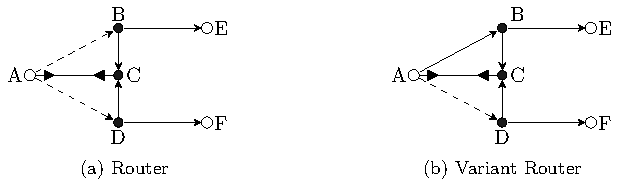
\includegraphics[width=.7\textwidth]{Router.pdf}
\caption{Example of connector complementary refinement }\label{fig:EXrefine}
\end{figure}
\begin{example}
In this example, we will take the well-known \emph{Exclusive Router} into consideration. This connector and one possible variant are shown in Figure~\ref{fig:EXrefine}. The \emph{variant router} is defined with only one major difference: one of the two \emph{LossySync} channels in the Exclusive Router is replaced with a \emph{Sync} channel. Therefore, the behavior of the variant router is actually not exclusive and all data items will be transported to node \emph{E} rather than being transmitted to node \emph{E} or \emph{F} exclusively in the original router. Notice that the variant router is a refinement of the original router and conversely not. \liyi{We construct} these two connectors first and set a concrete bound 10. We invoke the function \texttt{isRefinementOf} in both directions, i.e., \texttt{c2.isRefinementOf(c1, 10), c1.isRefinementOf(c2, 10)} where \texttt{c2} is the variant router. The results Z3 yields are \texttt{True} and \texttt{False} \liyi{up to bound $10$} (together with a counter example) respectively, which are consistent with our intuition.
The counter example is omitted here and the complete results including the counter example can be found at \cite{reo2coq2Z3}.
\end{example}

\begin{figure}[htb]
\centering
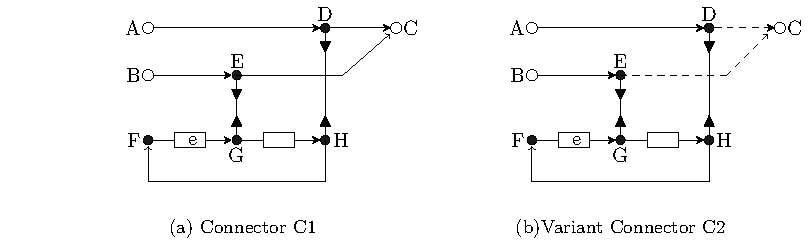
\includegraphics[width=.8\textwidth]{sequencer.pdf}
\caption{Example of connector complementary refinement}
\label{fig:large}
\end{figure}
\begin{example}
Figure~\ref{fig:large} shows an example of the application of a two-node sequencer, with the addition of a pair of \emph{Sync} channels and a \emph{SyncDrain} channel connecting each of the nodes of the sequencer to the nodes
\emph{A} and \emph{C}, and \emph{B} and \emph{C}, respectively. The leftmost channel of the sequencer is initialized to have a data item in its buffer, as indicated by the presence of the symbol \emph{e} in the box, which is actually a \emph{FIFO1e} channel. As the sequencer ensures that the take operations on nodes \emph{G} and \emph{H} can succeed only in the strict left-to-right order, the behavior of the connector $C1$ can be seen as imposing an order on the flow of the data items written to \emph{A} and \emph{B}. The timed data stream obtained by successive take operations on \emph{C} consists of the first data item written to \emph{B}, followed by the first data item written to \emph{A}, followed by the second data item written to \emph{B}, and so on. The variant connector $C2$ is obtained by replacing the pair of \emph{Sync} channels with a pair of one \emph{Sync} channel and one \emph{LossySync} channel. On account of the behavior of \emph{LossySync} channel, the first data item written to \emph{B} can be lost, which leads to the failure of the sequence order. Thus, the variant connector $C2$ is not a refinement of the original connector $C1$, but the original connector is indeed a refinement of the variant connector. The details of the concrete construction and the counter example are left out. The results Z3 solver presented are \texttt{False} for \texttt{c2.isRefinementOf(c1, 10)} and \texttt{True} for \texttt{c1.isRefinementOf(c2, 10)}, which are consistent with the results of theoretical deduction.

Comparing the behavior of connector $C1$ described in this example with the \emph{alternator} in Section \ref{sec:verification}, the data stream obtained on \emph{C} is made up of the data items written to \emph{B} and \emph{A} alternately for both connectors. Intuitively, the two connectors have the same behavior and thus are equivalent. Nevertheless, by constructing the connectors and executing the function \texttt{isRefinementOf} in both directions, the returned results are both \texttt{False}, which is contrary to our expectation. In fact, the reason for this result is that the constraints on the input nodes of the two connectors are different. \emph{SyncDrain} channel of \emph{alternator} ensures that the input time on nodes \emph{A} and \emph{B} are equal. However, the application of \emph{Sequencer} guarantees \liyi{that the time for} the two input nodes must be different. We can see that Z3 helps to avoid possible artificial mistakes by this example, which makes the advantage of Z3 more evident.


\end{example}

\subsection{Z3 as complement of Coq}
In the \liyi{previous assessments} of the refinement and equivalence relations or other properties in Coq, the \liyi{main constraint} is that users \liyi{need to be able to build a proof}. Furthermore, various behavioral properties or relations on infinite timed data streams can be proven, which makes Coq sufficiently powerful. Besides, the connectors whose properties have been proved can be regarded as theorems or lemmas to assist in proving properties of much larger ones. Recall that the main reason of introducing Z3 solver is that \xy{Coq cannot provide the proof of complementary refinement checking, i.e., one connector is not a refinement of the other one, or provide counter examples automatically. Coq users need to build the counter example manually to show that the property is not satisfiable.}

As we have seen, Z3 solver has shone light on complementary refinement checking. Besides, Z3 solver is much easier to use after the definition of the function \texttt{isRefinementOf} and the construction framework of Reo connectors, compared with using specific tactics and strategies in Coq. Moreover, counter examples can be provided \xy{as additional diagnostic feedback} while the refinement checking process returns \texttt{False}.
%Soundness and completeness of proofs in Z3 solver need a careful thought.
\xy{The main drawback of Z3 solver is the failure of providing ideally infinite timed data streams as witnesses for refinement relations.} A finite prefix of timed data stream is not enough to ensure the refinement relation between two Reo connectors for certain. As a result, the equivalence relation is also not ensured completely. Nevertheless, \xy{it has no influence on the complementary refinement checking. Once Z3 presents a counter example, the complementary refinement checking is finished, which is ensured by the aforementioned soundness of counter example generation using Algorithm 1.}
%As for time complexity, the efficiency of Z3 solver is well-known. The complexity of the counter-example generation algorithm is the formalization of Reo connectors in
\xy{However, we have shown that a bounded counter example is sufficient to prove the inexistence of refinement/equivalence relations and the bound in our experiments is usually less than 10. When checking complementary refinement relation, the experiments show that a bound limit around 5 can guarantee a proper counter example to be given in a reasonable time for many cases.}

\section{Conclusion and Future Work}\label{sec:conclusion}
In this paper, we present a new approach to model and reason about connectors in Coq and Z3. The model naturally
preserves the original structure of connectors. This also makes the connector description reasonably readable. We
implement the proof of properties for connectors using identified techniques and tactics provided by Coq. Properties are
defined in terms of predicates which provide an appropriate description of the relation among different
timed data streams on the nodes of a connector. All the analysis and verification work are based on the logical framework
where basic channels are viewed as axioms and composition operations are viewed as operators. As we can address
the relation among different timed data streams, we can reason about various properties including equivalence and refinement relations for connectors. Furthermore, since Coq cannot decide if a proposition is provable or not, we can also use Z3 to search for possible bounded counter examples automatically. Although in this paper we focus on refinement checking as an example, this approach can be applied to verification of various properties.

As some of the benefits of this approach are inherited from Coq, our approach has got some of its drawbacks as well.
The main limitation is that the analysis needs much more tactics and techniques when the constructor becomes large.
In the future work, we plan to enhance our framework by two different approaches.
\xy{
  Firstly, we are working on automating the proofs of Reo connector properties. In \cite{Foclasa17SCP} (which is an extended version of \cite{Foclasa17}), we developed an approach to generate Coq tactics automatically based on neural networks, which also works on all the proved theorems in this paper. We are looking for more efficient network structures and algorithms to improve the performance of this approach.
  }
Secondly, more attention is needed to precisely
evaluate how expressive this approach is for modeling temporal properties.

\subsection*{Acknowledgement}
\noindent The work was partially supported by the National Natural Science Foundation of China under grant no. 61772038, 61532019 and 61272160.

%\bibliographystyle{abbrv}
%\bibliography{the}
\begin{thebibliography}{ 10}
\expandafter\ifx\csname url\endcsname\relax
  \def\url#1{\texttt{#1}}\fi
\expandafter\ifx\csname urlprefix\endcsname\relax\def\urlprefix{URL }\fi
\expandafter\ifx\csname href\endcsname\relax
  \def\href#1#2{#2} \def\path#1{#1}\fi

\bibitem{reo2coq2Z3}
Package of source files.
\newblock \url{https://github.com/liyi-david/reo-z3}.

\bibitem{AAA+09}
B.~K. Aichernig, F.~Arbab, L.~Astefanoaei, F.~S. de~Boer, M.~Sun, and
  J.~Rutten.
\newblock {Fault-based Test Case Generation for Component Connectors.}
\newblock In {\em {Proceedings of TASE 2009}}, pages 147--154. IEEE Computer
  Society, 2009.

\bibitem{Arb04}
F.~Arbab.
\newblock {Reo: A Channel-based Coordination Model for Component Composition.}
\newblock {\em {Mathematical Structures in Computer Science}}, 14(3):329--366,
  2004.

\bibitem{AR03}
F.~Arbab and J.~Rutten.
\newblock {A Coinductive Calculus of Component Connectors.}
\newblock In {\em Proceedings of WADT 2002}, volume 2755 of {\em LNCS}, pages 34--55.
  Springer-Verlag, 2003.

\bibitem{BBK+10}
C.~Baier, T.~Blechmann, J.~Klein, S.~Kl{\"u}ppelholz, and W.~Leister.
\newblock {Design and Verification of Systems with Exogenous Coordination Using
  Vereofy.}
\newblock In {\em Proceedings of ISoLA 2010}, volume 6416 of {\em LNCS}, pages
  97--111. Springer, 2010.

\bibitem{BSAR06}
C.~Baier, M.~Sirjani, F.~Arbab, and J.~Rutten.
\newblock {Modeling Component Connectors in Reo by Constraint Automata.}
\newblock {\em {Science of Computer Programming}}, 61:75--113, 2006.

\bibitem{CCA04}
D.~Clarke, D.~Costa, and F.~Arbab.
\newblock {Modelling Coordination in Biological Systems.}
\newblock In {\em Proceedings of ISoLA'04}, volume 4313 of {\em LNCS}, pages
  9--25. Springer, 2004.

\bibitem{MouraB08}
L.~M. de~Moura and N.~Bj{\o}rner.
\newblock {Z3: an Efficient SMT Solver.}
\newblock In {\em Proceedings of TACAS 2008}, volume 4963 of {\em LNCS}, pages
  337--340. Springer, 2008.

\bibitem{RE98}
W.-P. de~Roever and K.~Engelhardt.
\newblock {\em {Data Refinement: Model-Oriented Proof Methods and their
  Comparison}}.
\newblock {Cambridge University Press}, 1998.

\bibitem{huet1997coq}
G.~Huet, G.~Kahn, and C.~Paulin-Mohring.
\newblock {The Coq Proof Assistant A Tutorial.}
\newblock {\em Rapport Technique}, 178, 1997.

\bibitem{Jon90}
C.~B. Jones.
\newblock {\em Systematic Software Development using {VDM}}.
\newblock Prentice-Hall, 1990.

\bibitem{JA12}
S.~T.~Q. Jongmans and F.~Arbab.
\newblock {Overview of Thirty Semantic Formalisms for Reo.}
\newblock {\em Scientific Annals of Computer Science}, 22(1):201--251, 2012.

\bibitem{KSA+08}
R.~Khosravi, M.~Sirjani, N.~Asoudeh, S.~Sahebi, and H.~Iravanchi.
\newblock {Modeling and Analysis of Reo Connectors Using Alloy.}
\newblock In {\em Proceedings of COORDINATION 2008}, volume 5052 of {\em LNCS},
  pages 169--183. Springer, 2008.

\bibitem{KB09}
S.~Kl{\"u}ppelholz and C.~Baier.
\newblock {Symbolic Model Checking for Channel-based Component Connectors}.
\newblock {\em Science of Computer Programming}, 74(9):688--701, 2009.

\bibitem{KKV12}
N.~Kokash, C.~Krause, and E.~de~Vink.
\newblock {Reo+mCRL2: A Framework for Model-checking Dataflow in Service
  Compositions}.
\newblock {\em {Formal Aspects of Computing}}, 24:187--216, 2012.

\bibitem{LS15}
Y.~Li and M.~Sun.
\newblock {Modeling and Verification of Component Connectors in Coq}.
\newblock {\em Science of Computer Programming}, 113(3):285--301, 2015.

\bibitem{Ros98}
A.~W. Roscoe.
\newblock {\em {The Theory and Practice of Concurrency}}.
\newblock Prentice Hall, 1998.

\bibitem{Sun12}
M.~Sun.
\newblock {Connectors as Designs: The Time Dimension.}
\newblock In {\em Proceedings of TASE 2012}, pages 201--208. IEEE Computer
  Society, 2012.

\bibitem{SA07}
M.~Sun and F.~Arbab.
\newblock {Web Services Choreography and Orchestration in Reo and Constraint
  Automata}.
\newblock In {\em {Proceedings of SAC'07}}, pages 346--353. ACM, 2007.

\bibitem{SAA+12}
M.~Sun, F.~Arbab, B.~K. Aichernig, L.~Astefanoaei, F.~S. de~Boer, and
  J.~Rutten.
\newblock {Connectors as Designs: Modeling, Refinement and Test Case
  Generation}.
\newblock {\em Science of Computer Programming}, 77(7-8):799--822, 2012.

\bibitem{ZHL+17}
X.~Zhang, W.~Hong, Y.~Li, and M.~Sun.
\newblock {Reasoning About Connectors in Coq}.
\newblock In {\em {Proceedings of FACS 2016 }}, volume 10231 of {\em {LNCS}},
  pages {172--190}. {Springer}, 2017.

\bibitem{Foclasa17}
W.~Hong, S.~Nawaz, X.~Zhang, Y.~Li and M.~Sun.
\newblock {Using Coq for Formal Modeling and Verification of Timed Connectors}.
\newblock In {Software Engineering and Formal Methods: SEFM 2017 Collocated Workshops, Revised Selected Papers},
volumn 10729 of {\em {LNCS}},
 pages {558-573}. {Springer}, 2018.

\bibitem{Foclasa17SCP}
Y.~Li, X.~Zhang, W.~Hong, S.~Nawaz and M.~Sun.
\newblock {Using Coq and Recurrent Neural Network to Model and Verify Timed Connectors}.
\newblock submitted to {\em Science of Computer Programming}.


\end{thebibliography}


\end{document}
